\chapter{Planning and Task Clarification}

This chapter delves into the process of planning and clarifying tasks for the prototype, as depicted in Figure \ref{fig:planning} following Pahl and Beitz's model. As mentioned previously in Chapter \ref{ch:methodicproductdevelopment} this step play a critical role in the product development process. They involve precisely defining and understanding the requirements and expectations related to a specific task or project. The aim is to remove any confusion and ensure that everyone involved has a shared understanding of what needs to be achieved.

\begin{figure}[ht!]
    \centering
    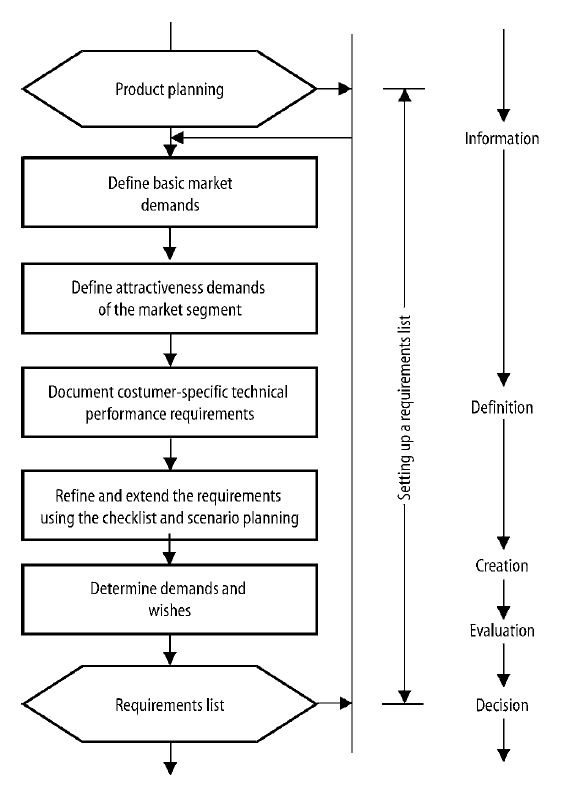
\includegraphics[width=0.6\textwidth]{texs/Part1/chapter2/image/planning.png}
    \caption{Planning and Task Clarification \cite{Pahl07m}}
    \label{fig:planning}
\end{figure}

During this step, the specific goals, limitations, and things that need to be produced for the task are identified \cite{Pahl07a}. By clarifying and specifying tasks, engineers and designers set a strong foundation for the later stages of product development. This allows them to move forward with a clear sense of direction and focus. To achieve this, Pahl and Beitz formulated a series of questions that must be answered to ensure that the task is well-defined and understood \cite{Pahl07a}. These questions are:

\begin{itemize}
    \item What is the objectives of the solution?
    \item What characteristics should the solution have?
    \item What characteristics should the solution avoid?
\end{itemize}

By answering these questions, the requirements for the solution can be identified and spelled out. These requirements will serve as the basis for the subsequent phases of the product development process. The outcome of this step is a list of requirements that outline the needs, expectations, and restrictions tied to the task \cite{Pahl07a}.

\section{Establishing the Prototype's Requirements}
To properly establish the requirements for the prototype, it is suggested to propely define the objectives of the prototype and clearly divide them into demands and wishes \cite{Pahl07n}.

Demands, as described by Pahl and Beitz \cite{Pahl07n}, are the essential and non-negotiable requirements that must be fulfilled for the product to be considered successful. They represent the core functionality and characteristics that the product must possess to meet its intended purpose and provide value to the users. Demands are typically based on objective criteria and are crucial for ensuring the product's basic functionality and compliance.

On the other hand, wishes are defined as the desirable but non-essential requirements or features that stakeholders would like to see in the product. Wishes often involve additional functionalities, aesthetics, or user experience enhancements that would provide added value or differentiate the product in the market. While wishes may not be mandatory, they can contribute to customer satisfaction, competitive advantage, and overall product excellence.

In addition, all of the requirements defined is possible must be quantifiable. This means that the requirements must be measurable and testable. This is important for ensuring that the requirements are met and that the product is able to fulfill its intended purpose.


\section{Identifying the Prototype's Requirements}
In this section, the requirements of the prototype will be established. The checklist (see Figure \ref{fig:checklist}) will be used as a guideline to ensure that all the requirements are properly identified and defined.

\begin{figure}[ht!]
    \centering
    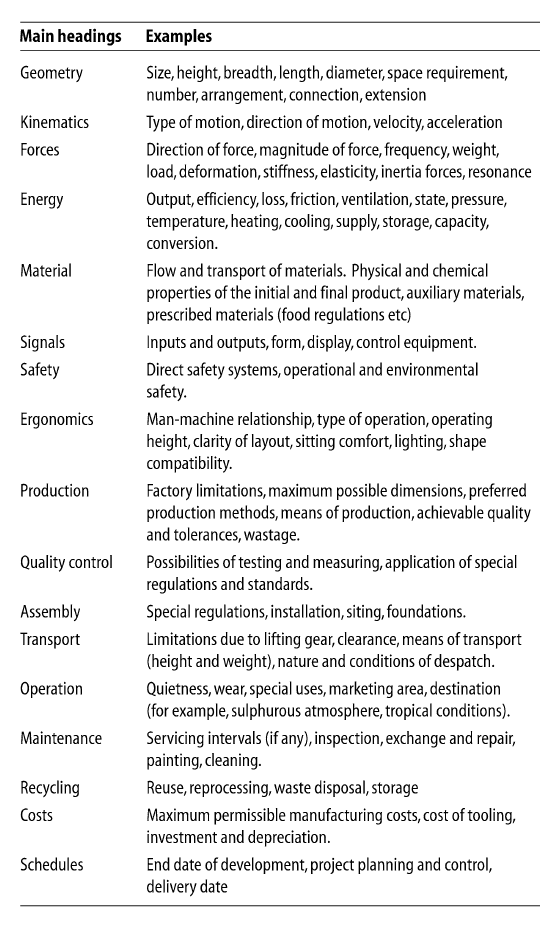
\includegraphics[width=0.6\textwidth]{texs/Part1/chapter2/image/requirements.png}
    \caption{Checklist for Establishing the Prototype's Requirements \cite{Pahl07o}}
    \label{fig:checklist}
\end{figure}

\subsection{Geometry}
When creating a prototype, it's crucial to get its size and shape right so that people can use it effectively. The size determines how big the prototype is and how well it functions. However, we need to be mindful not to make the prototype too large due to manufacturing limitations.

For our prototype, we're utilizing a 3D printing service provided by TH Brandenburg. We're specifically using the Original Prusa i3 MK3S+ 3D printer, which has a maximum printing area of 210 mm by 210 mm by 250 mm \cite{Prusa}. This means we have to work within these size constraints.

To ensure that our prototype fits within these limits, we've decided to slightly reduce its size. We're making it about 10\% smaller than the maximum printing area. This adjustment ensures that our prototype can be comfortably accommodated on the 3D printer at TH Brandenburg. Given these considerations, the largest dimensions we've chosen for the prototype are 190 mm by 190 mm by 220 mm.

\subsection{Energy}
The energy needed for the prototype is really important because it affects how useful and convenient it is. We\'ve made a requirement that the prototype should be able to work on its own for at least 1 hour using the provided power supply. This rule is in place to make sure the prototype can work by itself and give users a smooth experience.

By being able to work for at least 1 hour, the prototype shows that it can keep running for a reasonable amount of time without needing to be charged often or relying on outside power. This enables users to operate the device without concern for an extended period, offering more opportunities to explore its functionality and capabilities. It also provides users with the freedom to engage with the prototype in real-life scenarios, offering valuable insights into its performance and effectiveness.

\subsection{Forces}
The force requirement for the prototype has two main aspects: ensuring it can handle the weight of its components while also adhering to a maximum weight limit.

Firstly, it's crucial to verify that the prototype can effectively support the weight of its components without compromising its overall structure or functionality. This ensures the prototype's durability and ability to withstand the forces exerted by its components. Additionally, it guarantees that the prototype can be manipulated and operated without the risk of damage or malfunction.

Furthermore, there is a specific constraint that the total weight of the prototype must not surpass 2 kg. This encompasses the collective weight of all internal components, including both the predefined components and any additional materials integrated during the design process. Adhering to this weight limit ensures the prototype remains lightweight and manageable, while still meeting the intended performance criteria.

\subsection{Materials}
When crafting the prototype, it's crucial to carefully consider the specific materials and components that will be used. In this project, there are certain components that have already been chosen, and they must be included to meet the requirements. These components include the Raspberry Pi 4B, a 7-inch touch screen, the Raspberry Pi Camera V2, and the Veektomx 10000mAh power bank.

These chosen components act as essential building blocks for the prototype's function and performance. The Raspberry Pi 4B, a versatile single-board computer, supplies computing power and functions as the core control unit for the prototype. The 7-inch touch screen enhances user interaction by providing a responsive and user-friendly interface for input and output.

The Raspberry Pi Camera V2 enables the capture of images and videos, allowing for a range of applications within the prototype. Lastly, the Veektomx 10000mAh power bank provides a dependable power source, ensuring continuous operation of the prototype.

\subsection{Ergonomics}
When it comes to ergonomics, the prototype has specific demands concerning its dimensions, mass, and how users hold it. First and foremost, the prototype needs to be compact and lightweight. This guarantees that it's easy to carry around, making it simple to handle and move. By minimizing the prototype's size and weight, it enhances user comfort and convenience during use.

Furthermore, a vital aspect of the ergonomics requirement is that users should be able to hold the prototype comfortably. This involves thinking about the prototype's shape, grip, and balance to ensure it's easy and secure to hold. The design should fit naturally into the contours of the user's hand, ensuring a stable and ergonomic grip. By optimizing the prototype's shape and considering user ergonomics, it can deliver a smooth and user-friendly experience.

\subsection{Production}
The production requirement for the prototype focuses on the manufacturing process and the materials used. The prototype must be designed to be manufactured using 3D printing technology. This ensures that the prototype can be produced using the available resources and capabilities. In addition, the prototype must be designed to be manufactured using PLA filament. This material is readily available and offers a good balance of strength and flexibility, making it suitable for the prototype's requirements.

\subsection{Operation}
The operation requirement for the prototype encompasses two key aspects: the ability to be used freehand and the capability to integrate with a tripod for improved stability.

Firstly, the prototype must be designed to facilitate freehand operation. This means that users should be able to interact with and operate the prototype comfortably and conveniently without the need for additional support or mounting. The design should consider ergonomic factors such as grip, button placement, and user-friendly controls, ensuring that users can manipulate the prototype easily and intuitively.

Secondly, the prototype should be capable of integrating with a tripod for enhanced stability when necessary. This feature allows users to attach the prototype securely to a tripod, providing a stable and stationary setup. By integrating tripod compatibility, the prototype can cater to scenarios where steady and controlled operation or positioning is required, such as capturing images or conducting experiments that demand minimal movement.

\subsection{Assembly}
The assembly requirement for the prototype emphasizes the importance of considering the ease of assembly and disassembly of its components. This design consideration enables users to access the inner components easily, facilitating maintenance and repair tasks.

By designing the prototype with ease of assembly in mind, it becomes simpler for users to put the components together without requiring complex tools or specialized knowledge. This promotes user-friendliness and reduces the time and effort required for initial assembly or subsequent modifications. Similarly, easy disassembly allows users to access the internal components when needed, simplifying troubleshooting, repairs, or component replacements.

Additionally, if feasible, the parts of the prototype should be designed with swappable properties. This means that individual components or modules can be easily removed and replaced, without the need to disassemble the entire prototype. Swappable parts enhance modularity, flexibility, and cost-effectiveness, as users can upgrade or replace specific components as needed, rather than replacing the entire prototype.

\subsection{Costs}
The cost requirement for the prototype focuses on the total cost of production. The prototype must be designed to be manufactured within a budget of 100 euros excluding the cost of the predefined components. This budget encompasses the cost of all materials and components used in the production process. By adhering to this cost limitation, the prototype can be produced within the available resources and capabilities.

\subsection{Schedules}
The schedule requirement for the prototype focuses on the time required for production. The prototype must be designed to be manufactured within a time frame of 2 weeks. This time frame encompasses the entire production process, from design to assembly. By adhering to this schedule, the prototype can be produced within the available resources and capabilities.

\subsection{Durability}
The durability requirement for the prototype includes considerations for resistance to dust and water, if feasible. While it may not always be possible to achieve complete resistance, efforts should be made to enhance the prototype's durability in these aspects.

Regarding dust resistance, the prototype should be designed to minimize the ingress of dust particles into its internal components and sensitive areas. This involves employing appropriate seals, filters, or protective enclosures to prevent dust from adversely affecting the prototype's performance or functionality. By reducing the risk of dust accumulation, the prototype can maintain its optimal operation and extend its lifespan.

In terms of water resistance, if feasible and relevant to the intended use, the prototype should exhibit a level of protection against water ingress. This can involve incorporating waterproof or water-resistant materials, seals, or coatings to shield the internal components from moisture. Ensuring water resistance enhances the prototype's durability and enables usage in environments where exposure to water or humidity is likely.

\section{Requirement List}
Table 1 and Table 2 on the following pages show the requirements list which included the requirements described in this chapter.
